% Options for packages loaded elsewhere
\PassOptionsToPackage{unicode}{hyperref}
\PassOptionsToPackage{hyphens}{url}
%
\documentclass[
  ignorenonframetext,
]{beamer}
\usepackage{pgfpages}
\setbeamertemplate{caption}[numbered]
\setbeamertemplate{caption label separator}{: }
\setbeamercolor{caption name}{fg=normal text.fg}
\beamertemplatenavigationsymbolsempty
% Prevent slide breaks in the middle of a paragraph
\widowpenalties 1 10000
\raggedbottom
\setbeamertemplate{part page}{
  \centering
  \begin{beamercolorbox}[sep=16pt,center]{part title}
    \usebeamerfont{part title}\insertpart\par
  \end{beamercolorbox}
}
\setbeamertemplate{section page}{
  \centering
  \begin{beamercolorbox}[sep=12pt,center]{part title}
    \usebeamerfont{section title}\insertsection\par
  \end{beamercolorbox}
}
\setbeamertemplate{subsection page}{
  \centering
  \begin{beamercolorbox}[sep=8pt,center]{part title}
    \usebeamerfont{subsection title}\insertsubsection\par
  \end{beamercolorbox}
}
\AtBeginPart{
  \frame{\partpage}
}
\AtBeginSection{
  \ifbibliography
  \else
    \frame{\sectionpage}
  \fi
}
\AtBeginSubsection{
  \frame{\subsectionpage}
}
\usepackage{lmodern}
\usepackage{amsmath}
\usepackage{ifxetex,ifluatex}
\ifnum 0\ifxetex 1\fi\ifluatex 1\fi=0 % if pdftex
  \usepackage[T1]{fontenc}
  \usepackage[utf8]{inputenc}
  \usepackage{textcomp} % provide euro and other symbols
  \usepackage{amssymb}
\else % if luatex or xetex
  \usepackage{unicode-math}
  \defaultfontfeatures{Scale=MatchLowercase}
  \defaultfontfeatures[\rmfamily]{Ligatures=TeX,Scale=1}
\fi
% Use upquote if available, for straight quotes in verbatim environments
\IfFileExists{upquote.sty}{\usepackage{upquote}}{}
\IfFileExists{microtype.sty}{% use microtype if available
  \usepackage[]{microtype}
  \UseMicrotypeSet[protrusion]{basicmath} % disable protrusion for tt fonts
}{}
\makeatletter
\@ifundefined{KOMAClassName}{% if non-KOMA class
  \IfFileExists{parskip.sty}{%
    \usepackage{parskip}
  }{% else
    \setlength{\parindent}{0pt}
    \setlength{\parskip}{6pt plus 2pt minus 1pt}}
}{% if KOMA class
  \KOMAoptions{parskip=half}}
\makeatother
\usepackage{xcolor}
\IfFileExists{xurl.sty}{\usepackage{xurl}}{} % add URL line breaks if available
\IfFileExists{bookmark.sty}{\usepackage{bookmark}}{\usepackage{hyperref}}
\hypersetup{
  pdftitle={APLA\_Replication\_Code\_Presentation},
  pdfauthor={Omar Hammoud Gallego},
  hidelinks,
  pdfcreator={LaTeX via pandoc}}
\urlstyle{same} % disable monospaced font for URLs
\newif\ifbibliography
\usepackage{color}
\usepackage{fancyvrb}
\newcommand{\VerbBar}{|}
\newcommand{\VERB}{\Verb[commandchars=\\\{\}]}
\DefineVerbatimEnvironment{Highlighting}{Verbatim}{commandchars=\\\{\}}
% Add ',fontsize=\small' for more characters per line
\usepackage{framed}
\definecolor{shadecolor}{RGB}{248,248,248}
\newenvironment{Shaded}{\begin{snugshade}}{\end{snugshade}}
\newcommand{\AlertTok}[1]{\textcolor[rgb]{0.94,0.16,0.16}{#1}}
\newcommand{\AnnotationTok}[1]{\textcolor[rgb]{0.56,0.35,0.01}{\textbf{\textit{#1}}}}
\newcommand{\AttributeTok}[1]{\textcolor[rgb]{0.77,0.63,0.00}{#1}}
\newcommand{\BaseNTok}[1]{\textcolor[rgb]{0.00,0.00,0.81}{#1}}
\newcommand{\BuiltInTok}[1]{#1}
\newcommand{\CharTok}[1]{\textcolor[rgb]{0.31,0.60,0.02}{#1}}
\newcommand{\CommentTok}[1]{\textcolor[rgb]{0.56,0.35,0.01}{\textit{#1}}}
\newcommand{\CommentVarTok}[1]{\textcolor[rgb]{0.56,0.35,0.01}{\textbf{\textit{#1}}}}
\newcommand{\ConstantTok}[1]{\textcolor[rgb]{0.00,0.00,0.00}{#1}}
\newcommand{\ControlFlowTok}[1]{\textcolor[rgb]{0.13,0.29,0.53}{\textbf{#1}}}
\newcommand{\DataTypeTok}[1]{\textcolor[rgb]{0.13,0.29,0.53}{#1}}
\newcommand{\DecValTok}[1]{\textcolor[rgb]{0.00,0.00,0.81}{#1}}
\newcommand{\DocumentationTok}[1]{\textcolor[rgb]{0.56,0.35,0.01}{\textbf{\textit{#1}}}}
\newcommand{\ErrorTok}[1]{\textcolor[rgb]{0.64,0.00,0.00}{\textbf{#1}}}
\newcommand{\ExtensionTok}[1]{#1}
\newcommand{\FloatTok}[1]{\textcolor[rgb]{0.00,0.00,0.81}{#1}}
\newcommand{\FunctionTok}[1]{\textcolor[rgb]{0.00,0.00,0.00}{#1}}
\newcommand{\ImportTok}[1]{#1}
\newcommand{\InformationTok}[1]{\textcolor[rgb]{0.56,0.35,0.01}{\textbf{\textit{#1}}}}
\newcommand{\KeywordTok}[1]{\textcolor[rgb]{0.13,0.29,0.53}{\textbf{#1}}}
\newcommand{\NormalTok}[1]{#1}
\newcommand{\OperatorTok}[1]{\textcolor[rgb]{0.81,0.36,0.00}{\textbf{#1}}}
\newcommand{\OtherTok}[1]{\textcolor[rgb]{0.56,0.35,0.01}{#1}}
\newcommand{\PreprocessorTok}[1]{\textcolor[rgb]{0.56,0.35,0.01}{\textit{#1}}}
\newcommand{\RegionMarkerTok}[1]{#1}
\newcommand{\SpecialCharTok}[1]{\textcolor[rgb]{0.00,0.00,0.00}{#1}}
\newcommand{\SpecialStringTok}[1]{\textcolor[rgb]{0.31,0.60,0.02}{#1}}
\newcommand{\StringTok}[1]{\textcolor[rgb]{0.31,0.60,0.02}{#1}}
\newcommand{\VariableTok}[1]{\textcolor[rgb]{0.00,0.00,0.00}{#1}}
\newcommand{\VerbatimStringTok}[1]{\textcolor[rgb]{0.31,0.60,0.02}{#1}}
\newcommand{\WarningTok}[1]{\textcolor[rgb]{0.56,0.35,0.01}{\textbf{\textit{#1}}}}
\usepackage{graphicx}
\makeatletter
\def\maxwidth{\ifdim\Gin@nat@width>\linewidth\linewidth\else\Gin@nat@width\fi}
\def\maxheight{\ifdim\Gin@nat@height>\textheight\textheight\else\Gin@nat@height\fi}
\makeatother
% Scale images if necessary, so that they will not overflow the page
% margins by default, and it is still possible to overwrite the defaults
% using explicit options in \includegraphics[width, height, ...]{}
\setkeys{Gin}{width=\maxwidth,height=\maxheight,keepaspectratio}
% Set default figure placement to htbp
\makeatletter
\def\fps@figure{htbp}
\makeatother
\setlength{\emergencystretch}{3em} % prevent overfull lines
\providecommand{\tightlist}{%
  \setlength{\itemsep}{0pt}\setlength{\parskip}{0pt}}
\setcounter{secnumdepth}{-\maxdimen} % remove section numbering
\ifluatex
  \usepackage{selnolig}  % disable illegal ligatures
\fi

\title{APLA\_Replication\_Code\_Presentation}
\author{Omar Hammoud Gallego}
\date{19/11/2020}

\begin{document}
\frame{\titlepage}

\begin{frame}[fragile]{Upload Packages and Data}
\protect\hypertarget{upload-packages-and-data}{}
\begin{Shaded}
\begin{Highlighting}[]
\CommentTok{\# Upload Packages for Data analysis and Map}
\FunctionTok{library}\NormalTok{(}\StringTok{"dplyr"}\NormalTok{)}
\FunctionTok{library}\NormalTok{(}\StringTok{"ggplot2"}\NormalTok{)}
\FunctionTok{theme\_set}\NormalTok{(}\FunctionTok{theme\_bw}\NormalTok{())}
\FunctionTok{library}\NormalTok{(}\StringTok{"sf"}\NormalTok{)}
\FunctionTok{library}\NormalTok{(}\StringTok{"tmap"}\NormalTok{)}
\FunctionTok{library}\NormalTok{(}\StringTok{"rnaturalearth"}\NormalTok{)}
\FunctionTok{library}\NormalTok{(}\StringTok{"rnaturalearthdata"}\NormalTok{)}
\FunctionTok{library}\NormalTok{(}\StringTok{"tidyr"}\NormalTok{)}
\FunctionTok{library}\NormalTok{(}\StringTok{"stringr"}\NormalTok{)  }\CommentTok{\# To do text analysis }

\CommentTok{\# For color}
\FunctionTok{library}\NormalTok{(}\StringTok{"RColorBrewer"}\NormalTok{)}
\FunctionTok{library}\NormalTok{(}\StringTok{"viridis"}\NormalTok{)}
\FunctionTok{library}\NormalTok{(}\StringTok{"ggrepel"}\NormalTok{) }\CommentTok{\# might be useful later}

\CommentTok{\# Plot all titles in ggplot2 centered}
\FunctionTok{theme\_update}\NormalTok{(}\AttributeTok{plot.title =} \FunctionTok{element\_text}\NormalTok{(}\AttributeTok{hjust =} \FloatTok{0.5}\NormalTok{))}
\end{Highlighting}
\end{Shaded}

\begin{Shaded}
\begin{Highlighting}[]
\CommentTok{\# Set Working Directory}
\CommentTok{\#setwd("C:/Users/omarh/Desktop/")}

\CommentTok{\# Upload APLA Database}
\NormalTok{APLA}\OtherTok{\textless{}{-}}\NormalTok{ APLA}\SpecialCharTok{::}\NormalTok{APLA\_Database }

\CommentTok{\# Upload Data for Refugee Numbers only}
\NormalTok{APLA\_Data\_1}\OtherTok{\textless{}{-}}\NormalTok{ APLA}\SpecialCharTok{::}\NormalTok{Data\_Refugees\_UNHCR         }\CommentTok{\# Data APLA  }

\CommentTok{\# Upload Data to Map All Countries Latin America}
\NormalTok{APLA\_Map}\OtherTok{\textless{}{-}}\NormalTok{ APLA}\SpecialCharTok{::}\NormalTok{APLA\_Map                      }\CommentTok{\# Data APLA for Mapping }
\end{Highlighting}
\end{Shaded}
\end{frame}

\begin{frame}[fragile]{Calculate Regulatory Complexity and
Liberalisation}
\protect\hypertarget{calculate-regulatory-complexity-and-liberalisation}{}
\begin{Shaded}
\begin{Highlighting}[]
\CommentTok{\#APLA\textless{}{-} read.csv("APLA\_Database.csv")}
\CommentTok{\#summary(APLA)}

\CommentTok{\# Transform as Tibble}
\NormalTok{APLA\_T }\OtherTok{\textless{}{-}} \FunctionTok{as\_tibble}\NormalTok{(APLA)}
\CommentTok{\#APLA\_T}

\CommentTok{\# Filter out columns on international agreements}
\NormalTok{APLA\_T1}\OtherTok{\textless{}{-}}\NormalTok{ APLA\_T }\SpecialCharTok{\%\textgreater{}\%} \FunctionTok{select}\NormalTok{(}\DecValTok{1}\NormalTok{,}\DecValTok{2}\NormalTok{, }\DecValTok{35}\SpecialCharTok{:}\DecValTok{262}\NormalTok{)}

\CommentTok{\# Only Questions of Liberalisation and Comments included}
\NormalTok{APLA\_T2}\OtherTok{\textless{}{-}}\NormalTok{ APLA\_T1 }\SpecialCharTok{\%\textgreater{}\%} \FunctionTok{select}\NormalTok{(}\DecValTok{1}\NormalTok{,}\DecValTok{2}\NormalTok{, }\FunctionTok{ends\_with}\NormalTok{(}\FunctionTok{c}\NormalTok{(}\StringTok{"2\_1"}\NormalTok{,}\StringTok{"3\_1\_1"}\NormalTok{)))}

\CommentTok{\# Select only commentary section to calculate number "Art" to calculate Regulatory Complexity}
\NormalTok{APLA\_T3}\OtherTok{\textless{}{-}}\NormalTok{ APLA\_T2 }\SpecialCharTok{\%\textgreater{}\%}
  \FunctionTok{select}\NormalTok{(}\DecValTok{1}\NormalTok{,}\DecValTok{2}\NormalTok{, }\FunctionTok{ends\_with}\NormalTok{(}\StringTok{"3\_1\_1"}\NormalTok{))}

\CommentTok{\# Delete of first row}
\NormalTok{APLA\_T3}\OtherTok{=}\NormalTok{ APLA\_T3[}\SpecialCharTok{{-}}\DecValTok{1}\NormalTok{,]}

\CommentTok{\# Pivot Table for data manipulation}
\NormalTok{APLA\_T\_L }\OtherTok{\textless{}{-}} \FunctionTok{pivot\_longer}\NormalTok{(APLA\_T3, }\AttributeTok{cols =} \FunctionTok{colnames}\NormalTok{(APLA\_T3)[}\DecValTok{3}\SpecialCharTok{:}\FunctionTok{length}\NormalTok{(}\FunctionTok{colnames}\NormalTok{(APLA\_T3))],}
                        \AttributeTok{names\_to =} \StringTok{"Question"}\NormalTok{, }\AttributeTok{values\_to =} \StringTok{"Comment"}\NormalTok{)}

\CommentTok{\# Transform variable from factor to string}
\NormalTok{APLA\_T\_L}\SpecialCharTok{$}\NormalTok{Comment}\OtherTok{\textless{}{-}} \FunctionTok{as.character}\NormalTok{(APLA\_T\_L}\SpecialCharTok{$}\NormalTok{Comment)}

\CommentTok{\# Value 1 if "Art" present "0" otherwise}
\NormalTok{APLA\_T\_L1}\OtherTok{\textless{}{-}}\NormalTok{ APLA\_T\_L }\SpecialCharTok{\%\textgreater{}\%}
  \FunctionTok{mutate}\NormalTok{(}\AttributeTok{Included=} \FunctionTok{ifelse}\NormalTok{(}\FunctionTok{grepl}\NormalTok{(}\StringTok{"Art"}\NormalTok{, APLA\_T\_L}\SpecialCharTok{$}\NormalTok{Comment), }\DecValTok{1}\NormalTok{,}\DecValTok{0}\NormalTok{))}

\CommentTok{\# Aggregate values of Included per Country, Year, and Question}
\NormalTok{APLA\_T\_L2}\OtherTok{\textless{}{-}}\NormalTok{ APLA\_T\_L1 }\SpecialCharTok{\%\textgreater{}\%}
  \FunctionTok{group\_by}\NormalTok{(Q1,Q2) }\SpecialCharTok{\%\textgreater{}\%}
  \FunctionTok{summarise}\NormalTok{(}\AttributeTok{Frequency=} \FunctionTok{sum}\NormalTok{(Included))}

\CommentTok{\# Calculate Percentage by looking at number of "Included" per Country/Year as a \% of total number of indicators = 57}
\NormalTok{APLA\_T\_L3}\OtherTok{\textless{}{-}}\NormalTok{ APLA\_T\_L2 }\SpecialCharTok{\%\textgreater{}\%}
    \FunctionTok{mutate}\NormalTok{(}\AttributeTok{Total=}\DecValTok{57}\NormalTok{) }\SpecialCharTok{\%\textgreater{}\%}
    \FunctionTok{mutate}\NormalTok{(}\AttributeTok{Regulatory\_Complexity=}\NormalTok{ Frequency}\SpecialCharTok{/}\NormalTok{Total}\SpecialCharTok{*}\DecValTok{100}\NormalTok{) }

\CommentTok{\# Round Regulatory Complexity}
\NormalTok{APLA\_T\_L3}\SpecialCharTok{$}\NormalTok{Regulatory\_Complexity}\OtherTok{\textless{}{-}} \FunctionTok{round}\NormalTok{(APLA\_T\_L3}\SpecialCharTok{$}\NormalTok{Regulatory\_Complexity)}

\CommentTok{\# Rename Country and Year, and Year transformed in numeric}
\FunctionTok{colnames}\NormalTok{(APLA\_T\_L3)[}\DecValTok{1}\NormalTok{] }\OtherTok{\textless{}{-}} \StringTok{"Country"}
\FunctionTok{colnames}\NormalTok{(APLA\_T\_L3)[}\DecValTok{2}\NormalTok{] }\OtherTok{\textless{}{-}} \StringTok{"Year"}
\NormalTok{APLA\_T\_L3}\SpecialCharTok{$}\NormalTok{Year}\OtherTok{\textless{}{-}} \FunctionTok{as.numeric}\NormalTok{(}\FunctionTok{as.character}\NormalTok{(APLA\_T\_L3}\SpecialCharTok{$}\NormalTok{Year))}
\end{Highlighting}
\end{Shaded}

\begin{Shaded}
\begin{Highlighting}[]
\CommentTok{\# Run Regulatory Complexity Code First}

\CommentTok{\# Only Questions of Liberalisation and Comments included}
\NormalTok{APLA\_T4}\OtherTok{\textless{}{-}}\NormalTok{ APLA\_T1 }\SpecialCharTok{\%\textgreater{}\%} \FunctionTok{select}\NormalTok{(}\DecValTok{1}\NormalTok{,}\DecValTok{2}\NormalTok{, }\FunctionTok{ends\_with}\NormalTok{(}\FunctionTok{c}\NormalTok{(}\StringTok{"2\_1"}\NormalTok{)))}

\CommentTok{\# Delete of first row}
\NormalTok{APLA\_T4}\OtherTok{=}\NormalTok{ APLA\_T4[}\SpecialCharTok{{-}}\DecValTok{1}\NormalTok{,]}

\CommentTok{\# Pivot Table for data manipulation}
\NormalTok{APLA\_T\_L4 }\OtherTok{\textless{}{-}} \FunctionTok{pivot\_longer}\NormalTok{(APLA\_T4, }\AttributeTok{cols =} \FunctionTok{colnames}\NormalTok{(APLA\_T4)[}\DecValTok{3}\SpecialCharTok{:}\FunctionTok{length}\NormalTok{(}\FunctionTok{colnames}\NormalTok{(APLA\_T4))],}
                        \AttributeTok{names\_to =} \StringTok{"Question"}\NormalTok{, }\AttributeTok{values\_to =} \StringTok{"Liberalisation\_Score"}\NormalTok{)}

\CommentTok{\# Mutate Liberalisation Score into numeric}
\NormalTok{APLA\_T\_L4}\SpecialCharTok{$}\NormalTok{Liberalisation\_Score}\OtherTok{\textless{}{-}} \FunctionTok{as.numeric}\NormalTok{(}\FunctionTok{as.character}\NormalTok{(APLA\_T\_L4}\SpecialCharTok{$}\NormalTok{Liberalisation\_Score, }\AttributeTok{na.rm=} \ConstantTok{TRUE}\NormalTok{))}
\NormalTok{APLA\_T\_L4}\SpecialCharTok{$}\NormalTok{Question}\OtherTok{\textless{}{-}} \FunctionTok{as.factor}\NormalTok{(APLA\_T\_L4}\SpecialCharTok{$}\NormalTok{Question)}

\NormalTok{APLA\_T\_L4[}\FunctionTok{complete.cases}\NormalTok{(APLA\_T\_L4),]}
\end{Highlighting}
\end{Shaded}

\begin{verbatim}
## # A tibble: 19,623 x 4
##    Q1        Q2    Question Liberalisation_Score
##    <fct>     <fct> <fct>                   <dbl>
##  1 Argentina 1990  Q54.2_1                     0
##  2 Argentina 1990  LA3.2_1                     1
##  3 Argentina 1990  LA7.2_1                     1
##  4 Argentina 1990  LA41.2_1                    0
##  5 Argentina 1990  LA43.2_1                    1
##  6 Argentina 1990  LA53.2_1                    0
##  7 Argentina 1990  LA59.2_1                    1
##  8 Argentina 1991  Q54.2_1                     0
##  9 Argentina 1991  LA3.2_1                     1
## 10 Argentina 1991  LA7.2_1                     1
## # ... with 19,613 more rows
\end{verbatim}

\begin{Shaded}
\begin{Highlighting}[]
\CommentTok{\# Aggregate values of Included per Country, Year, and Question}
\NormalTok{APLA\_T\_L5}\OtherTok{\textless{}{-}}\NormalTok{ APLA\_T\_L4 }\SpecialCharTok{\%\textgreater{}\%}
  \FunctionTok{na.omit}\NormalTok{() }\SpecialCharTok{\%\textgreater{}\%}
  \FunctionTok{group\_by}\NormalTok{(Q1,Q2) }\SpecialCharTok{\%\textgreater{}\%}
  \FunctionTok{summarise}\NormalTok{(}\AttributeTok{Liberal\_Policies=} \FunctionTok{sum}\NormalTok{(Liberalisation\_Score }\SpecialCharTok{==} \DecValTok{0}\NormalTok{), }\AttributeTok{Restrictive\_Policies=} \FunctionTok{sum}\NormalTok{(Liberalisation\_Score }\SpecialCharTok{==} \DecValTok{1}\NormalTok{)) }\SpecialCharTok{\%\textgreater{}\%}
  \FunctionTok{mutate}\NormalTok{(}\AttributeTok{Sum\_Both =}\NormalTok{ Liberal\_Policies }\SpecialCharTok{+}\NormalTok{ Restrictive\_Policies) }\SpecialCharTok{\%\textgreater{}\%}
  \FunctionTok{mutate}\NormalTok{(}\AttributeTok{Liberalisation=}\NormalTok{ Liberal\_Policies}\SpecialCharTok{/}\NormalTok{ Sum\_Both)}
  
\CommentTok{\# Round Liberalisation}
\NormalTok{APLA\_T\_L5}\SpecialCharTok{$}\NormalTok{Liberalisation}\OtherTok{\textless{}{-}} \FunctionTok{round}\NormalTok{(APLA\_T\_L5}\SpecialCharTok{$}\NormalTok{Liberalisation, }\AttributeTok{digits =} \DecValTok{2}\NormalTok{)}

\CommentTok{\# Take only values where Total\_Both =\textgreater{} 9}
\NormalTok{APLA\_T\_L6}\OtherTok{\textless{}{-}}\NormalTok{ APLA\_T\_L5[APLA\_T\_L5}\SpecialCharTok{$}\NormalTok{Sum\_Both }\SpecialCharTok{\textgreater{}=} \DecValTok{9}\NormalTok{, ]}

\CommentTok{\# Rename Country and Year, and Year transformed in numeric}
\FunctionTok{colnames}\NormalTok{(APLA\_T\_L6)[}\DecValTok{1}\NormalTok{] }\OtherTok{\textless{}{-}} \StringTok{"Country"}
\FunctionTok{colnames}\NormalTok{(APLA\_T\_L6)[}\DecValTok{2}\NormalTok{] }\OtherTok{\textless{}{-}} \StringTok{"Year"}
\NormalTok{APLA\_T\_L6}\SpecialCharTok{$}\NormalTok{Year}\OtherTok{\textless{}{-}} \FunctionTok{as.numeric}\NormalTok{(}\FunctionTok{as.character}\NormalTok{(APLA\_T\_L6}\SpecialCharTok{$}\NormalTok{Year))}
\end{Highlighting}
\end{Shaded}
\end{frame}

\begin{frame}[fragile]{Plot Number of Refugees in Latin America,
Regulatory Complexity and Liberalisation over Time}
\protect\hypertarget{plot-number-of-refugees-in-latin-america-regulatory-complexity-and-liberalisation-over-time}{}
\begin{Shaded}
\begin{Highlighting}[]
\CommentTok{\# Check and change class variable refugees}
\CommentTok{\#class(APLA\_Data\_1$RefugeeAndLikeSit)}
\NormalTok{APLA\_Data\_1}\SpecialCharTok{$}\NormalTok{RefugeeAndLikeSit}\OtherTok{\textless{}{-}} \FunctionTok{as.numeric}\NormalTok{(APLA\_Data\_1}\SpecialCharTok{$}\NormalTok{RefugeeAndLikeSit)}

\CommentTok{\# Calculate maximum number of Refugees in each country (not used)}
\NormalTok{APLA\_Data\_1 }\SpecialCharTok{\%\textgreater{}\%}
\FunctionTok{group\_by}\NormalTok{(Country) }\SpecialCharTok{\%\textgreater{}\%} \FunctionTok{summarize}\NormalTok{(}\AttributeTok{m =} \FunctionTok{max}\NormalTok{(RefugeeAndLikeSit))}
\end{Highlighting}
\end{Shaded}

\begin{verbatim}
## # A tibble: 20 x 2
##    Country                 m
##    <fct>               <dbl>
##  1 Argentina           11901
##  2 Bolivia               787
##  3 Brazil              20783
##  4 Chile                2001
##  5 Colombia              478
##  6 Costa Rica         276210
##  7 Cuba                   NA
##  8 Dominican Republic     NA
##  9 Ecuador            264907
## 10 El Salvador         20300
## 11 Guatemala          233236
## 12 Honduras           237100
## 13 Mexico             360991
## 14 Nicaragua           16000
## 15 Panama              17665
## 16 Paraguay              250
## 17 Peru                 2466
## 18 Rest of Region      62269
## 19 Uruguay               349
## 20 Venezuela          204340
\end{verbatim}

\begin{Shaded}
\begin{Highlighting}[]
\CommentTok{\# Create new variable All Other Countries}
\NormalTok{APLA\_Data\_Filtered\_1}\OtherTok{\textless{}{-}}\NormalTok{ APLA\_Data\_1 }\SpecialCharTok{\%\textgreater{}\%}
    \FunctionTok{filter}\NormalTok{(Country }\SpecialCharTok{\%in\%} \FunctionTok{c}\NormalTok{(}\StringTok{"Costa Rica"}\NormalTok{,}\StringTok{"Ecuador"}\NormalTok{,}\StringTok{"Guatemala"}\NormalTok{,}\StringTok{"Honduras"}\NormalTok{,}\StringTok{"Mexico"}\NormalTok{,}\StringTok{"Venezuela"}\NormalTok{,}\StringTok{"Rest of Region"}\NormalTok{))}

\CommentTok{\# PLOT REFUGEE NUMBERS IN LATIN AMERICA}
\NormalTok{PLOT}\OtherTok{\textless{}{-}} \FunctionTok{ggplot}\NormalTok{(APLA\_Data\_Filtered\_1, }\FunctionTok{aes}\NormalTok{(Year, RefugeeAndLikeSit, }\AttributeTok{col=}\NormalTok{ Country)) }\SpecialCharTok{+}
  \FunctionTok{geom\_line}\NormalTok{()}\SpecialCharTok{+}
  \FunctionTok{facet\_wrap}\NormalTok{(}\SpecialCharTok{\textasciitilde{}}\NormalTok{ Country, }\AttributeTok{scales =} \StringTok{"free\_y"}\NormalTok{)}\SpecialCharTok{+}
  \FunctionTok{ggtitle}\NormalTok{(}\StringTok{"Refugees and People in Refugee{-}Like Situation in Latin America"}\NormalTok{)}\SpecialCharTok{+}
  \FunctionTok{ylab}\NormalTok{(}\StringTok{"Refugee Numbers"}\NormalTok{)}\SpecialCharTok{+}
  \FunctionTok{theme}\NormalTok{(}\AttributeTok{plot.title =} \FunctionTok{element\_text}\NormalTok{(}\StringTok{"serif"}\NormalTok{, }\AttributeTok{size =} \StringTok{"14"}\NormalTok{, }\AttributeTok{hjust =} \FloatTok{0.5}\NormalTok{))}\SpecialCharTok{+}
  \FunctionTok{theme\_bw}\NormalTok{()}

\CommentTok{\# PLOT WITH ADJUSTED LABELS}
\FunctionTok{require}\NormalTok{(scales)}
\NormalTok{PLOT }\SpecialCharTok{+} \FunctionTok{scale\_y\_continuous}\NormalTok{(}\AttributeTok{labels =}\NormalTok{ comma) }\SpecialCharTok{+} 
    \FunctionTok{scale\_x\_continuous}\NormalTok{(}\AttributeTok{breaks =} \FunctionTok{c}\NormalTok{(}\DecValTok{1990}\NormalTok{, }\DecValTok{2000}\NormalTok{, }\DecValTok{2010}\NormalTok{, }\DecValTok{2018}\NormalTok{))}\SpecialCharTok{+}
    \FunctionTok{theme}\NormalTok{(}\AttributeTok{legend.position =} \StringTok{"none"}\NormalTok{)}
\end{Highlighting}
\end{Shaded}

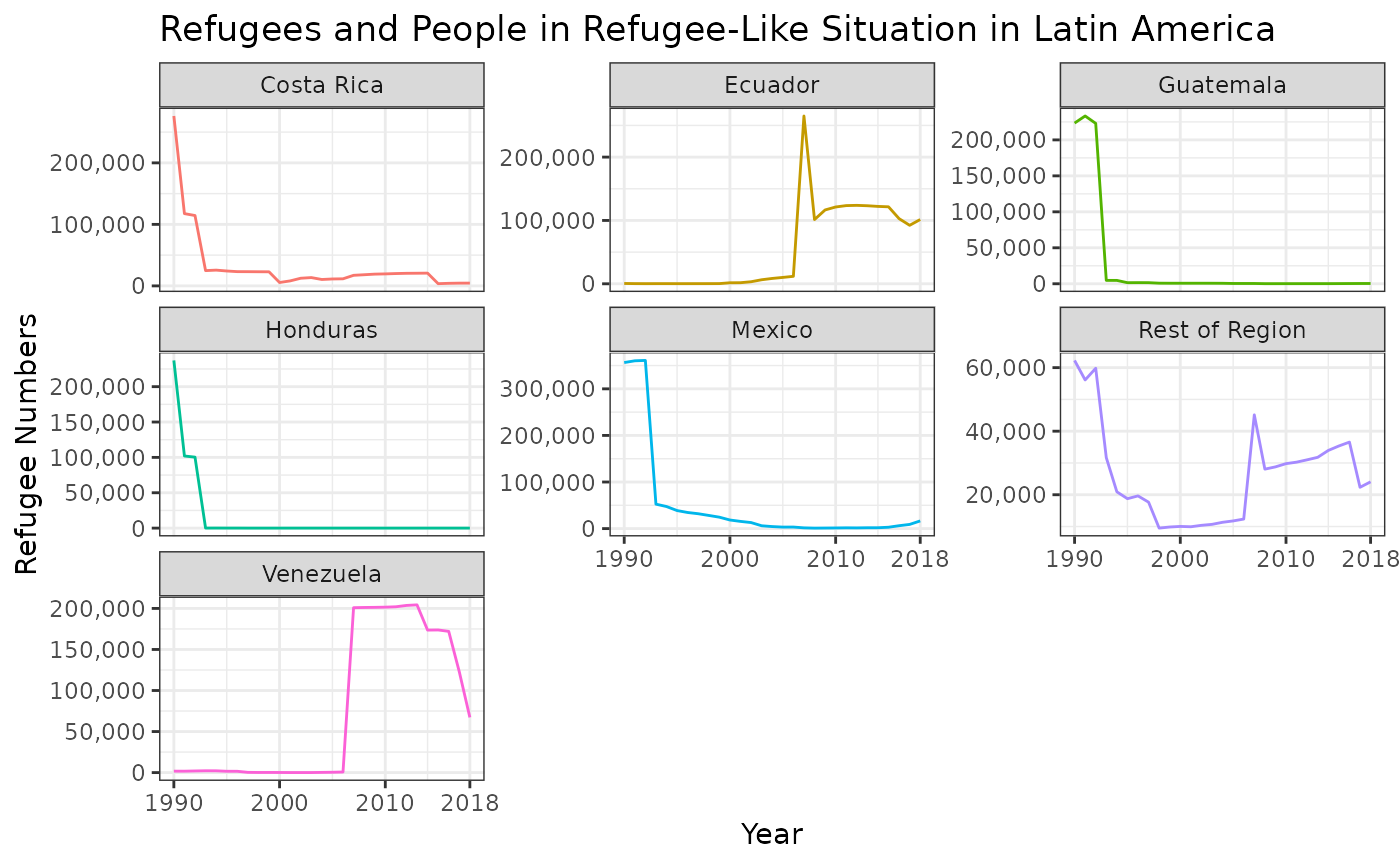
\includegraphics{APLA_Replication_Code_Presentation_files/figure-beamer/Refugees in LA-1.pdf}

\begin{Shaded}
\begin{Highlighting}[]
\FunctionTok{ggplot}\NormalTok{(APLA\_T\_L3, }\FunctionTok{aes}\NormalTok{(Year, Regulatory\_Complexity)) }\SpecialCharTok{+}
  \FunctionTok{geom\_jitter}\NormalTok{(}\AttributeTok{height=}\FloatTok{0.8}\NormalTok{, }\AttributeTok{width =} \FloatTok{0.7}\NormalTok{, }\FunctionTok{aes}\NormalTok{(}\AttributeTok{color=}\StringTok{"Country{-}Year"}\NormalTok{), }\AttributeTok{alpha=}\FloatTok{0.5}\NormalTok{, }\AttributeTok{size=}\DecValTok{2}\NormalTok{)}\SpecialCharTok{+}
  \FunctionTok{scale\_colour\_manual}\NormalTok{(}\AttributeTok{name=}\StringTok{\textquotesingle{}\textquotesingle{}}\NormalTok{, }\AttributeTok{values =} \FunctionTok{c}\NormalTok{(}\StringTok{"Locally Weighted Regression"}\OtherTok{=} \StringTok{"red"}\NormalTok{,}\StringTok{"Country{-}Year"}\OtherTok{=}\StringTok{"grey"}\NormalTok{, }\StringTok{"Linear Regression Line"}\OtherTok{=} \StringTok{"blue"}\NormalTok{))}\SpecialCharTok{+}
  \FunctionTok{geom\_smooth}\NormalTok{(}\AttributeTok{linetype=}\StringTok{"dashed"}\NormalTok{, }\FunctionTok{aes}\NormalTok{(}\AttributeTok{color=}\StringTok{"Locally Weighted Regression"}\NormalTok{), }\AttributeTok{se=}\ConstantTok{FALSE}\NormalTok{)}\SpecialCharTok{+}
  \FunctionTok{geom\_smooth}\NormalTok{(}\AttributeTok{method =} \StringTok{\textquotesingle{}lm\textquotesingle{}}\NormalTok{, }\AttributeTok{formula =}\NormalTok{ y}\SpecialCharTok{\textasciitilde{}}\NormalTok{x, }\FunctionTok{aes}\NormalTok{(}\AttributeTok{color=}\StringTok{"Linear Regression Line"}\NormalTok{), }\AttributeTok{se=}\ConstantTok{FALSE}\NormalTok{)}\SpecialCharTok{+}
  \FunctionTok{scale\_shape}\NormalTok{(}\AttributeTok{solid=}\ConstantTok{FALSE}\NormalTok{)}\SpecialCharTok{+}
  \FunctionTok{scale\_x\_continuous}\NormalTok{(}\AttributeTok{breaks =} \FunctionTok{c}\NormalTok{(}\DecValTok{1990}\NormalTok{, }\DecValTok{1995}\NormalTok{, }\DecValTok{2000}\NormalTok{, }\DecValTok{2005}\NormalTok{, }\DecValTok{2010}\NormalTok{, }\DecValTok{2015}\NormalTok{, }\DecValTok{2018}\NormalTok{))}\SpecialCharTok{+}
  \FunctionTok{theme\_bw}\NormalTok{()}\SpecialCharTok{+}
  \FunctionTok{ggtitle}\NormalTok{(}\StringTok{"Regulatory Complexity of Asylum Policies in Latin America"}\NormalTok{)}\SpecialCharTok{+}
  \FunctionTok{ylab}\NormalTok{(}\StringTok{"Regulatory Complexity"}\NormalTok{)}\SpecialCharTok{+}
  \FunctionTok{theme}\NormalTok{(}\AttributeTok{plot.title =} \FunctionTok{element\_text}\NormalTok{(}\StringTok{"serif"}\NormalTok{, }\AttributeTok{size =} \StringTok{"14"}\NormalTok{, }\AttributeTok{hjust =} \FloatTok{0.5}\NormalTok{))}\SpecialCharTok{+}
  \FunctionTok{theme}\NormalTok{(}\AttributeTok{legend.title =} \FunctionTok{element\_blank}\NormalTok{())}\SpecialCharTok{+}
  \FunctionTok{theme}\NormalTok{(}\AttributeTok{legend.key =} \FunctionTok{element\_rect}\NormalTok{(}\AttributeTok{fill =} \StringTok{"white"}\NormalTok{)) }\SpecialCharTok{+} \FunctionTok{guides}\NormalTok{(}\AttributeTok{color=}\FunctionTok{guide\_legend}\NormalTok{(}\AttributeTok{override.aes=}\FunctionTok{list}\NormalTok{(}\AttributeTok{fill=}\ConstantTok{NA}\NormalTok{))) }\CommentTok{\#+}
\end{Highlighting}
\end{Shaded}

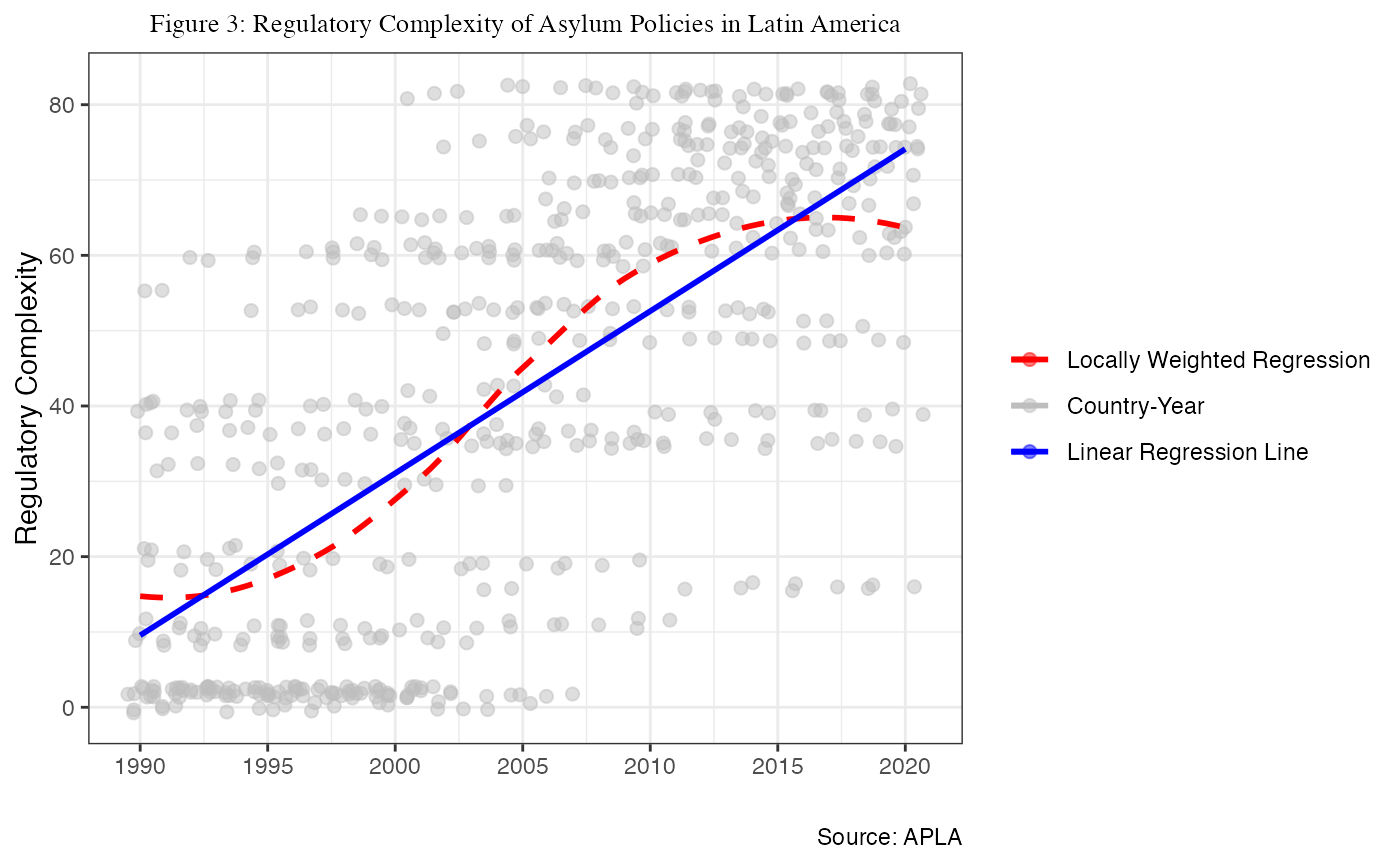
\includegraphics{APLA_Replication_Code_Presentation_files/figure-beamer/Regulatory Complexity Over Time-1.pdf}

\begin{Shaded}
\begin{Highlighting}[]
  \CommentTok{\#scale\_color\_brewer(palette="Dark2")}
\end{Highlighting}
\end{Shaded}

\begin{Shaded}
\begin{Highlighting}[]
\FunctionTok{ggplot}\NormalTok{(APLA\_T\_L3, }\FunctionTok{aes}\NormalTok{(Year, Regulatory\_Complexity, }\AttributeTok{col=}\NormalTok{ Country)) }\SpecialCharTok{+}
  \FunctionTok{geom\_line}\NormalTok{()}\SpecialCharTok{+}
  \FunctionTok{facet\_wrap}\NormalTok{(.}\SpecialCharTok{\textasciitilde{}}\NormalTok{ Country, }\AttributeTok{ncol=} \DecValTok{5}\NormalTok{)}\SpecialCharTok{+}
  \FunctionTok{theme}\NormalTok{(}\AttributeTok{legend.position =} \StringTok{"none"}\NormalTok{)}\SpecialCharTok{+}  \CommentTok{\# to remove legend}
  \FunctionTok{ggtitle}\NormalTok{(}\StringTok{"Regulatory Complexity in Asylum Policies across Latin America, 1990{-}2018"}\NormalTok{) }\SpecialCharTok{+}
  \FunctionTok{ylab}\NormalTok{(}\StringTok{"Regulatory Complexity"}\NormalTok{)}
\end{Highlighting}
\end{Shaded}

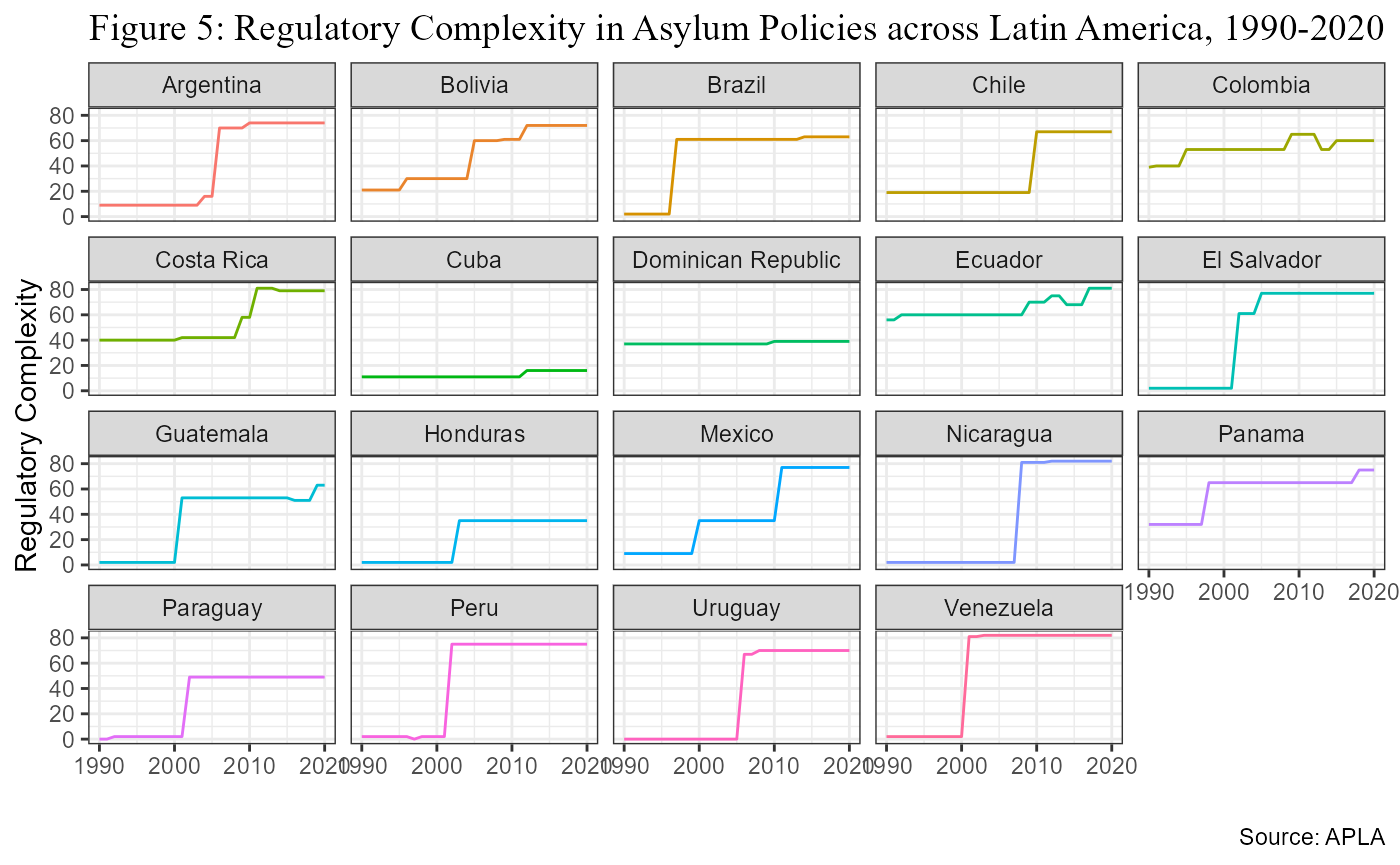
\includegraphics{APLA_Replication_Code_Presentation_files/figure-beamer/Plots of Development of Policy Over-Time Across Countries for Paper 1. Regulatory Complexity-1.pdf}
\end{frame}

\begin{frame}[fragile]{Plot Map of Countries Codified using APLA
Dataset}
\protect\hypertarget{plot-map-of-countries-codified-using-apla-dataset}{}
\begin{Shaded}
\begin{Highlighting}[]
\NormalTok{world }\OtherTok{\textless{}{-}} \FunctionTok{ne\_countries}\NormalTok{(}\AttributeTok{scale =} \StringTok{"medium"}\NormalTok{, }\AttributeTok{returnclass =} \StringTok{"sf"}\NormalTok{)   }\CommentTok{\# Map of World}
\CommentTok{\#class(world)}

\NormalTok{APLA\_Sel}\OtherTok{\textless{}{-}}\NormalTok{ APLA\_Map }\SpecialCharTok{\%\textgreater{}\%}                                       \CommentTok{\# Create Database with Selected Years for Plotting}
  \FunctionTok{filter}\NormalTok{(Year }\SpecialCharTok{\%in\%} \FunctionTok{c}\NormalTok{(}\StringTok{"1990"}\NormalTok{, }\StringTok{"2000"}\NormalTok{, }\StringTok{"2010"}\NormalTok{, }\StringTok{"2018"}\NormalTok{))}

\CommentTok{\# Rename column where names is "name", so that I can merge with my other dataset}
\FunctionTok{colnames}\NormalTok{(world)[}\DecValTok{4}\NormalTok{] }\OtherTok{\textless{}{-}} \StringTok{"Country"}

\CommentTok{\# VERY IMPORTANT TO MERGE MAP AND DATA }
\NormalTok{Map\_APLA\_Data}\OtherTok{\textless{}{-}} \FunctionTok{merge}\NormalTok{(APLA\_Sel, world, }\AttributeTok{by=}\StringTok{"Country"}\NormalTok{)}

\CommentTok{\# to transform MAP\_APLA from data frame into sf and data.frame}
\FunctionTok{st\_geometry}\NormalTok{(Map\_APLA\_Data) }\OtherTok{\textless{}{-}}\NormalTok{ Map\_APLA\_Data}\SpecialCharTok{$}\NormalTok{geometry}


\CommentTok{\# Display all countries codified so far + Compass + Scale Bar + labels changed!+ Title. USE THIS}
\FunctionTok{tm\_shape}\NormalTok{(Map\_APLA\_Data) }\SpecialCharTok{+} \FunctionTok{tm\_borders}\NormalTok{(}\StringTok{"black"}\NormalTok{, }\AttributeTok{lwd=}\NormalTok{ .}\DecValTok{5}\NormalTok{) }\SpecialCharTok{+} 
  \FunctionTok{tm\_layout}\NormalTok{(}\AttributeTok{title=}\StringTok{"1990{-}2018"}\NormalTok{, }\AttributeTok{title.size =} \FloatTok{1.5}\NormalTok{, }\AttributeTok{title.position =}\FunctionTok{c}\NormalTok{(}\FloatTok{0.6}\NormalTok{, }\StringTok{"top"}\NormalTok{)) }\SpecialCharTok{+} 
  \FunctionTok{tm\_polygons}\NormalTok{(}\StringTok{"Codified"}\NormalTok{, }\AttributeTok{title=}\StringTok{"Codified APLA Countries"}\NormalTok{, }\AttributeTok{palette=} \StringTok{"Blues"}\NormalTok{, }\AttributeTok{style=}\StringTok{"fixed"}\NormalTok{, }\AttributeTok{breaks=}\FunctionTok{c}\NormalTok{(}\DecValTok{0}\NormalTok{, }\FloatTok{0.1}\NormalTok{, }\DecValTok{1}\NormalTok{), }
              \AttributeTok{labels=}\FunctionTok{c}\NormalTok{(}\StringTok{"Not Codified"}\NormalTok{,}\StringTok{"Codified Countries"}\NormalTok{)) }\SpecialCharTok{+} \FunctionTok{tm\_compass}\NormalTok{(}\AttributeTok{position =} \FunctionTok{c}\NormalTok{(}\FloatTok{0.3}\NormalTok{, }\FloatTok{0.35}\NormalTok{)) }\SpecialCharTok{+} 
  \FunctionTok{tm\_scale\_bar}\NormalTok{(}\AttributeTok{width =} \FloatTok{0.22}\NormalTok{, }\AttributeTok{position =} \FunctionTok{c}\NormalTok{(}\FloatTok{0.65}\NormalTok{, }\FloatTok{0.08}\NormalTok{)) }
\end{Highlighting}
\end{Shaded}

\begin{figure}
\centering
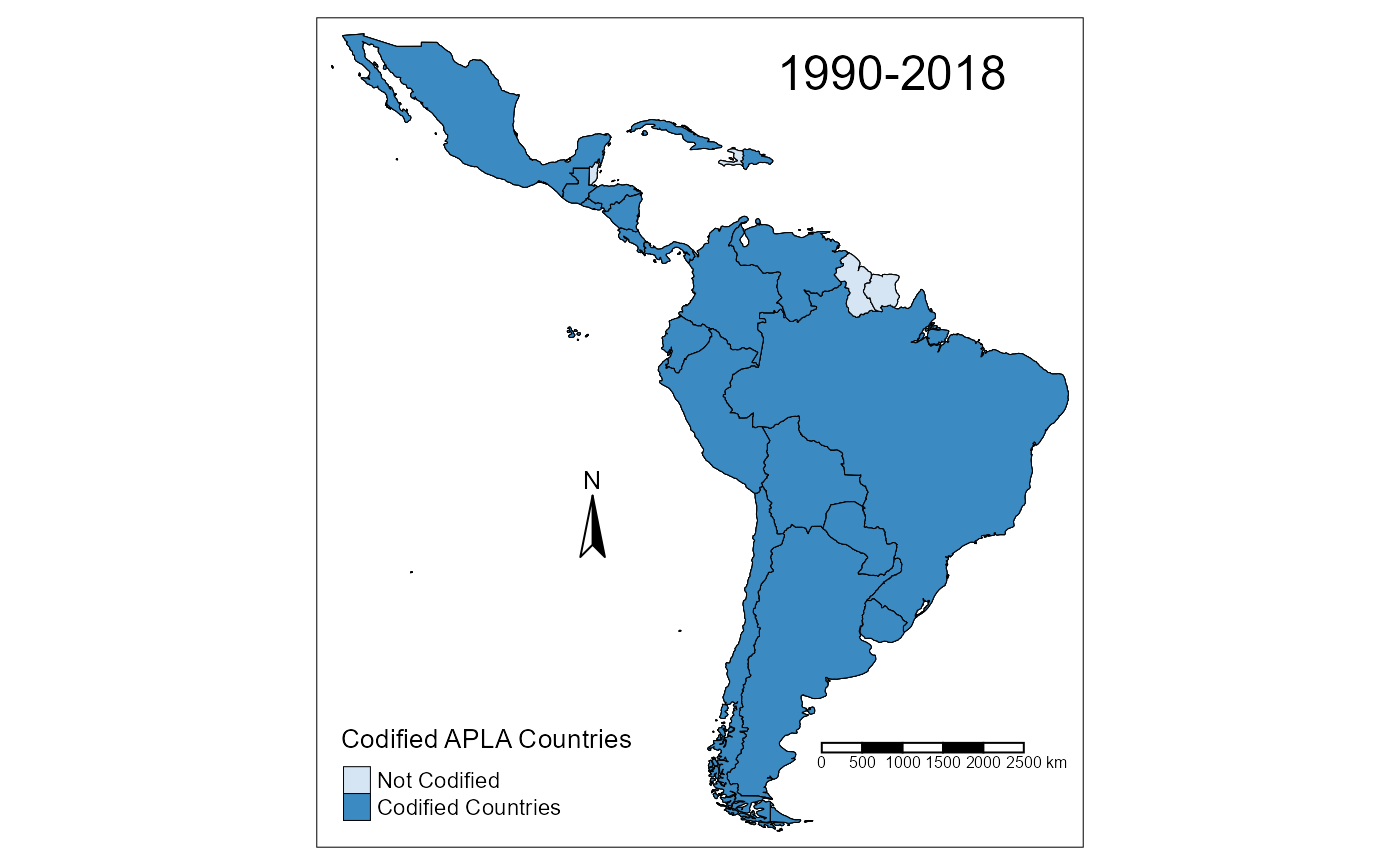
\includegraphics{APLA_Replication_Code_Presentation_files/figure-beamer/Map of Countries Codified APLA-1.pdf}
\caption{Source: APLA Database}
\end{figure}
\end{frame}

\begin{frame}[fragile]{Maps of Policy Measures Included in Legislation
1990 - 2018}
\protect\hypertarget{maps-of-policy-measures-included-in-legislation-1990---2018}{}
\begin{Shaded}
\begin{Highlighting}[]
\NormalTok{world }\OtherTok{\textless{}{-}} \FunctionTok{ne\_countries}\NormalTok{(}\AttributeTok{scale =} \StringTok{"medium"}\NormalTok{, }\AttributeTok{returnclass =} \StringTok{"sf"}\NormalTok{)}
\FunctionTok{class}\NormalTok{(world)}
\end{Highlighting}
\end{Shaded}

\begin{verbatim}
## [1] "sf"         "data.frame"
\end{verbatim}

\begin{Shaded}
\begin{Highlighting}[]
\CommentTok{\# Rename column where names is "name", so that I can merge with my other dataset}
\FunctionTok{colnames}\NormalTok{(APLA)[}\DecValTok{1}\NormalTok{] }\OtherTok{\textless{}{-}} \StringTok{"Name"}
\FunctionTok{colnames}\NormalTok{(APLA)[}\DecValTok{2}\NormalTok{] }\OtherTok{\textless{}{-}} \StringTok{"Year"}
\FunctionTok{colnames}\NormalTok{(world)[}\DecValTok{4}\NormalTok{] }\OtherTok{\textless{}{-}} \StringTok{"Name"}
  
\CommentTok{\# VERY IMPORTANT TO MERGE MAP AND DATA }
\NormalTok{Policy\_Maps}\OtherTok{\textless{}{-}} \FunctionTok{merge}\NormalTok{(APLA, world, }\AttributeTok{by=}\StringTok{"Name"}\NormalTok{)}

\CommentTok{\# to transform IMPALA from data frame into sf and data.frame}
\FunctionTok{st\_geometry}\NormalTok{(Policy\_Maps) }\OtherTok{\textless{}{-}}\NormalTok{ Policy\_Maps}\SpecialCharTok{$}\NormalTok{geometry}

\CommentTok{\# to add colour to map}
\FunctionTok{library}\NormalTok{(RColorBrewer)}
\CommentTok{\#display.brewer.all()}

\CommentTok{\# Create Database with Selected Years for Plotting}
\NormalTok{Policy\_Maps\_Filtered}\OtherTok{\textless{}{-}}\NormalTok{ Policy\_Maps }\SpecialCharTok{\%\textgreater{}\%}                                       
  \FunctionTok{filter}\NormalTok{(Year }\SpecialCharTok{\%in\%} \FunctionTok{c}\NormalTok{(}\StringTok{"1990"}\NormalTok{, }\StringTok{"2000"}\NormalTok{, }\StringTok{"2010"}\NormalTok{, }\StringTok{"2018"}\NormalTok{))}
\end{Highlighting}
\end{Shaded}

\begin{Shaded}
\begin{Highlighting}[]
\CommentTok{\# Cartagena Refugee Definition LA7}
\FunctionTok{tm\_shape}\NormalTok{(Policy\_Maps\_Filtered) }\SpecialCharTok{+} \FunctionTok{tm\_borders}\NormalTok{(}\StringTok{"black"}\NormalTok{, }\AttributeTok{lwd=}\NormalTok{ .}\DecValTok{5}\NormalTok{) }\SpecialCharTok{+} \FunctionTok{tm\_polygons}\NormalTok{(}\StringTok{"LA7.1\_1"}\NormalTok{, }\AttributeTok{title=}\StringTok{"Cartagena Refugee Definition"}\NormalTok{, }\AttributeTok{palette=} \StringTok{"Blues"}\NormalTok{, }\AttributeTok{style=}\StringTok{"fixed"}\NormalTok{, }\AttributeTok{breaks=}\FunctionTok{c}\NormalTok{(}\FloatTok{0.0}\NormalTok{, }\FloatTok{0.9}\NormalTok{, }\FloatTok{1.0}\NormalTok{), }\AttributeTok{labels=}\FunctionTok{c}\NormalTok{(}\StringTok{"Not Incorporated"}\NormalTok{,}\StringTok{"Cartagena Incorporated"}\NormalTok{)) }\SpecialCharTok{+} \FunctionTok{tm\_facets}\NormalTok{(}\AttributeTok{by =} \StringTok{"Year"}\NormalTok{)}
\end{Highlighting}
\end{Shaded}

\includegraphics{APLA_Replication_Code_Presentation_files/figure-beamer/Maps of Policy Measures included in Legislation-1.pdf}

\begin{Shaded}
\begin{Highlighting}[]
\CommentTok{\# Asylum into Constitution  LA3}
\FunctionTok{tm\_shape}\NormalTok{(Policy\_Maps\_Filtered) }\SpecialCharTok{+} \FunctionTok{tm\_borders}\NormalTok{(}\StringTok{"black"}\NormalTok{, }\AttributeTok{lwd=}\NormalTok{ .}\DecValTok{5}\NormalTok{) }\SpecialCharTok{+} \FunctionTok{tm\_polygons}\NormalTok{(}\StringTok{"LA3.1\_1"}\NormalTok{, }\AttributeTok{title=}\StringTok{"Asylum into Constitution"}\NormalTok{, }\AttributeTok{palette=} \StringTok{"Blues"}\NormalTok{, }\AttributeTok{style=}\StringTok{"fixed"}\NormalTok{, }\AttributeTok{breaks=}\FunctionTok{c}\NormalTok{(}\FloatTok{0.0}\NormalTok{, }\FloatTok{0.9}\NormalTok{, }\FloatTok{1.0}\NormalTok{), }\AttributeTok{labels=}\FunctionTok{c}\NormalTok{(}\StringTok{"Not Included"}\NormalTok{,}\StringTok{"Included into Constitution"}\NormalTok{)) }\SpecialCharTok{+} \FunctionTok{tm\_facets}\NormalTok{(}\AttributeTok{by =} \StringTok{"Year"}\NormalTok{)}
\end{Highlighting}
\end{Shaded}

\includegraphics{APLA_Replication_Code_Presentation_files/figure-beamer/Maps of Policy Measures included in Legislation-2.pdf}

\begin{Shaded}
\begin{Highlighting}[]
\CommentTok{\# First Country of Asylum  Q101}
\FunctionTok{tm\_shape}\NormalTok{(Policy\_Maps\_Filtered) }\SpecialCharTok{+} \FunctionTok{tm\_borders}\NormalTok{(}\StringTok{"black"}\NormalTok{, }\AttributeTok{lwd=}\NormalTok{ .}\DecValTok{5}\NormalTok{) }\SpecialCharTok{+} \FunctionTok{tm\_polygons}\NormalTok{(}\StringTok{"Q101.1\_1"}\NormalTok{, }\AttributeTok{title=}\StringTok{"First Country of Asylum Principle"}\NormalTok{, }\AttributeTok{palette=} \StringTok{"Blues"}\NormalTok{, }\AttributeTok{style=}\StringTok{"fixed"}\NormalTok{, }\AttributeTok{breaks=}\FunctionTok{c}\NormalTok{(}\FloatTok{0.0}\NormalTok{, }\FloatTok{0.9}\NormalTok{, }\FloatTok{1.0}\NormalTok{), }\AttributeTok{labels=}\FunctionTok{c}\NormalTok{(}\StringTok{"Not Included"}\NormalTok{,}\StringTok{"Included into Legislation"}\NormalTok{)) }\SpecialCharTok{+} \FunctionTok{tm\_facets}\NormalTok{(}\AttributeTok{by =} \StringTok{"Year"}\NormalTok{)}
\end{Highlighting}
\end{Shaded}

\includegraphics{APLA_Replication_Code_Presentation_files/figure-beamer/Maps of Policy Measures included in Legislation-3.pdf}

\begin{Shaded}
\begin{Highlighting}[]
\CommentTok{\# Right to Work q54}
\FunctionTok{tm\_shape}\NormalTok{(Policy\_Maps\_Filtered) }\SpecialCharTok{+} \FunctionTok{tm\_borders}\NormalTok{(}\StringTok{"black"}\NormalTok{, }\AttributeTok{lwd=}\NormalTok{ .}\DecValTok{5}\NormalTok{) }\SpecialCharTok{+} \FunctionTok{tm\_polygons}\NormalTok{(}\StringTok{"Q54.1\_1"}\NormalTok{, }\AttributeTok{title=}\StringTok{"Right to Work"}\NormalTok{, }\AttributeTok{palette=} \StringTok{"Blues"}\NormalTok{, }\AttributeTok{style=}\StringTok{"fixed"}\NormalTok{, }\AttributeTok{breaks=}\FunctionTok{c}\NormalTok{(}\FloatTok{0.0}\NormalTok{, }\FloatTok{0.9}\NormalTok{, }\FloatTok{1.0}\NormalTok{), }\AttributeTok{labels=}\FunctionTok{c}\NormalTok{(}\StringTok{"Not Included"}\NormalTok{,}\StringTok{"Included"}\NormalTok{)) }\SpecialCharTok{+} \FunctionTok{tm\_facets}\NormalTok{(}\AttributeTok{by =} \StringTok{"Year"}\NormalTok{)}
\end{Highlighting}
\end{Shaded}

\includegraphics{APLA_Replication_Code_Presentation_files/figure-beamer/Maps of Policy Measures included in Legislation-4.pdf}

\begin{Shaded}
\begin{Highlighting}[]
\CommentTok{\# No Penalisation for Illegal Entry LA13}
\FunctionTok{tm\_shape}\NormalTok{(Policy\_Maps\_Filtered) }\SpecialCharTok{+} \FunctionTok{tm\_borders}\NormalTok{(}\StringTok{"black"}\NormalTok{, }\AttributeTok{lwd=}\NormalTok{ .}\DecValTok{5}\NormalTok{) }\SpecialCharTok{+} \FunctionTok{tm\_polygons}\NormalTok{(}\StringTok{"LA13.1\_1"}\NormalTok{, }\AttributeTok{title=}\StringTok{"No Penalisation for Illegal Entry"}\NormalTok{, }\AttributeTok{palette=} \StringTok{"Blues"}\NormalTok{, }\AttributeTok{style=}\StringTok{"fixed"}\NormalTok{, }\AttributeTok{breaks=}\FunctionTok{c}\NormalTok{(}\FloatTok{0.0}\NormalTok{, }\FloatTok{0.9}\NormalTok{, }\FloatTok{1.0}\NormalTok{), }\AttributeTok{labels=}\FunctionTok{c}\NormalTok{(}\StringTok{"Not Included"}\NormalTok{,}\StringTok{"Included in Legislation"}\NormalTok{)) }\SpecialCharTok{+} \FunctionTok{tm\_facets}\NormalTok{(}\AttributeTok{by =} \StringTok{"Year"}\NormalTok{)}
\end{Highlighting}
\end{Shaded}

\includegraphics{APLA_Replication_Code_Presentation_files/figure-beamer/Maps of Policy Measures included in Legislation-5.pdf}

\begin{Shaded}
\begin{Highlighting}[]
\CommentTok{\# Is UNHCR represented in refugee status decision council LA53}
\FunctionTok{tm\_shape}\NormalTok{(Policy\_Maps\_Filtered) }\SpecialCharTok{+} \FunctionTok{tm\_borders}\NormalTok{(}\StringTok{"black"}\NormalTok{, }\AttributeTok{lwd=}\NormalTok{ .}\DecValTok{5}\NormalTok{) }\SpecialCharTok{+} \FunctionTok{tm\_polygons}\NormalTok{(}\StringTok{"LA53.1\_1"}\NormalTok{, }\AttributeTok{title=}\StringTok{"UNHCR representation in National Refugee Council"}\NormalTok{, }\AttributeTok{palette=} \StringTok{"Blues"}\NormalTok{, }\AttributeTok{style=}\StringTok{"fixed"}\NormalTok{, }\AttributeTok{breaks=}\FunctionTok{c}\NormalTok{(}\FloatTok{0.0}\NormalTok{, }\FloatTok{0.9}\NormalTok{, }\FloatTok{1.0}\NormalTok{), }\AttributeTok{labels=}\FunctionTok{c}\NormalTok{(}\StringTok{"Not Included"}\NormalTok{,}\StringTok{"Included in Legislation"}\NormalTok{)) }\SpecialCharTok{+} \FunctionTok{tm\_facets}\NormalTok{(}\AttributeTok{by =} \StringTok{"Year"}\NormalTok{)}
\end{Highlighting}
\end{Shaded}

\includegraphics{APLA_Replication_Code_Presentation_files/figure-beamer/Maps of Policy Measures included in Legislation-6.pdf}

\begin{Shaded}
\begin{Highlighting}[]
\CommentTok{\# Is UNHCR informed if negative last instance decision}
\FunctionTok{tm\_shape}\NormalTok{(Policy\_Maps\_Filtered) }\SpecialCharTok{+} \FunctionTok{tm\_borders}\NormalTok{(}\StringTok{"black"}\NormalTok{, }\AttributeTok{lwd=}\NormalTok{ .}\DecValTok{5}\NormalTok{) }\SpecialCharTok{+} \FunctionTok{tm\_polygons}\NormalTok{(}\StringTok{"LA57.1\_1"}\NormalTok{, }\AttributeTok{title=}\StringTok{"UNHCR informed if Negative Decision"}\NormalTok{, }\AttributeTok{palette=} \StringTok{"Blues"}\NormalTok{, }\AttributeTok{style=}\StringTok{"fixed"}\NormalTok{, }\AttributeTok{breaks=}\FunctionTok{c}\NormalTok{(}\FloatTok{0.0}\NormalTok{, }\FloatTok{0.9}\NormalTok{, }\FloatTok{1.0}\NormalTok{), }\AttributeTok{labels=}\FunctionTok{c}\NormalTok{(}\StringTok{"Not Included"}\NormalTok{,}\StringTok{"Included in Legislation"}\NormalTok{)) }\SpecialCharTok{+} \FunctionTok{tm\_facets}\NormalTok{(}\AttributeTok{by =} \StringTok{"Year"}\NormalTok{)}
\end{Highlighting}
\end{Shaded}

\includegraphics{APLA_Replication_Code_Presentation_files/figure-beamer/Maps of Policy Measures included in Legislation-7.pdf}

\begin{Shaded}
\begin{Highlighting}[]
\CommentTok{\# Reasonable Time Limit to Submit Appeal Request LA59}
\FunctionTok{tm\_shape}\NormalTok{(Policy\_Maps\_Filtered) }\SpecialCharTok{+} \FunctionTok{tm\_borders}\NormalTok{(}\StringTok{"black"}\NormalTok{, }\AttributeTok{lwd=}\NormalTok{ .}\DecValTok{5}\NormalTok{) }\SpecialCharTok{+} \FunctionTok{tm\_polygons}\NormalTok{(}\StringTok{"LA59.1\_1"}\NormalTok{, }\AttributeTok{title=}\StringTok{"Reasonable Time to Submit Appeal"}\NormalTok{, }\AttributeTok{palette=} \StringTok{"Blues"}\NormalTok{, }\AttributeTok{style=}\StringTok{"fixed"}\NormalTok{, }\AttributeTok{breaks=}\FunctionTok{c}\NormalTok{(}\FloatTok{0.0}\NormalTok{, }\FloatTok{0.9}\NormalTok{, }\FloatTok{1.0}\NormalTok{), }\AttributeTok{labels=}\FunctionTok{c}\NormalTok{(}\StringTok{"Less than 15 Days"}\NormalTok{,}\StringTok{"15 Days or More"}\NormalTok{)) }\SpecialCharTok{+} \FunctionTok{tm\_facets}\NormalTok{(}\AttributeTok{by =} \StringTok{"Year"}\NormalTok{)}
\end{Highlighting}
\end{Shaded}

\includegraphics{APLA_Replication_Code_Presentation_files/figure-beamer/Maps of Policy Measures included in Legislation-8.pdf}

\begin{Shaded}
\begin{Highlighting}[]
\CommentTok{\# Refugee Status due to Persecution based on Gender LA65 }
\FunctionTok{tm\_shape}\NormalTok{(Policy\_Maps\_Filtered) }\SpecialCharTok{+} \FunctionTok{tm\_borders}\NormalTok{(}\StringTok{"black"}\NormalTok{, }\AttributeTok{lwd=}\NormalTok{ .}\DecValTok{5}\NormalTok{) }\SpecialCharTok{+} \FunctionTok{tm\_polygons}\NormalTok{(}\StringTok{"LA65.1\_1"}\NormalTok{, }\AttributeTok{title=}\StringTok{"Persecution due to Gender"}\NormalTok{, }\AttributeTok{palette=} \StringTok{"Blues"}\NormalTok{, }\AttributeTok{style=}\StringTok{"fixed"}\NormalTok{, }\AttributeTok{breaks=}\FunctionTok{c}\NormalTok{(}\FloatTok{0.0}\NormalTok{, }\FloatTok{0.9}\NormalTok{, }\FloatTok{1.0}\NormalTok{), }\AttributeTok{labels=}\FunctionTok{c}\NormalTok{(}\StringTok{"Not Included"}\NormalTok{,}\StringTok{"Included in Legislation"}\NormalTok{)) }\SpecialCharTok{+} \FunctionTok{tm\_facets}\NormalTok{(}\AttributeTok{by =} \StringTok{"Year"}\NormalTok{)}
\end{Highlighting}
\end{Shaded}

\includegraphics{APLA_Replication_Code_Presentation_files/figure-beamer/Maps of Policy Measures included in Legislation-9.pdf}
\end{frame}

\end{document}
